%%%%%%%%%%%%%%%%%%%%%%%%%%%%%%%%%%%%%%%%%%%%%%%%%%%%%%%%%%%%%
% Bakom den här mallen står ett antal lärare och forskare   %
% Luleå tekniska universitet. Har du kommentarer eller      %
% önskemål så kontakta huvudförfattare Magnus Gustafsson    %
% på avdelningen tillämpad fysik.                           %
%%%%%%%%%%%%%%%%%%%%%%%%%%%%%%%%%%%%%%%%%%%%%%%%%%%%%%%%%%%%%

%%%%%%%%%%%%%%%%%%%%%%%%%%%%%%%%%%%%%%%%%%%%%%%%%%%%%%%%%%%%%
% -                       PREAMBLE                        - %
%%%%%%%%%%%%%%%%%%%%%%%%%%%%%%%%%%%%%%%%%%%%%%%%%%%%%%%%%%%%%
% I "Premable" definierar man hur dokumentet ska formateras.
% Eftersom att LaTeX är ett programmeringsspråk som 
% kompileras så måste man ha en syntax som tillåter att man
% skriver in kommentarer som inte tolkas av kompilatorn. Vid
% det här laget har du säkert redan insett att man i LaTeX
% gör det genom att inleda med ett procenttecken.

\documentclass[a4paper]{article}
% "\usepackage{}" laddar paket som styr formatering och gör
% användbara kommandon tillgängliga
\usepackage[margin=2cm]{geometry} % Ändra marginaler
\usepackage[utf8]{inputenc} % Teckenkodning - använd denna.
\usepackage[T1]{fontenc}    % Teckensnitt
\usepackage[swedish, provide=*]{babel} % För att skriva på Svenska
\usepackage{graphicx} % Bildhantering
    \graphicspath{{Images/}} % Relativ sökväg till bilder. I
    % detta fall en mapp/folder (titta till vänster) som heter
    % "Images".
\usepackage{caption} % Figur och tabelltext
\usepackage{mathtools, amsmath, amssymb} % Verktyg för matematik
\usepackage{siunitx} % Paket för tal, enheter och intervall.
% Ex. \num{1e6}, \SI{15,3}{Nm} och \SIrange{10}{20}{\celcius})
\sisetup{output-decimal-marker={,},range-phrase=--,
         range-units=single,exponent-product=\cdot} 
% Skriver du på engelska, byt till: output-decimail-marker={.}
\usepackage{verbatim} % Långa kommentarer programmeringskod etc.
\usepackage{hyperref} % Hyperlinks
    %\hypersetup{bookmarksopen=true, bookmarksopenlevel=0,
    %            linkcolor={blue}}

% För att referera kan man använda "biblatex" paketet
% Numeriska referenser gör man genom att:
\usepackage[backend=bibtex,style=numeric,
            bibencoding=ascii]{biblatex}
% APA-referenser: 
% \usepackage[style=apa,backend=biber]{biblatex} 
% \DeclareLanguageMapping{swedish}{swedish-apa} 
% Referenserna som ska inkluderas i "bibliography".
\addbibresource{references.bib} % Detta kommando specificerar
% filen som man har samlat sina referenser i. Man kan ladda ner
% referenser av olika slags format från de flesta tidskrifter.
% I detta fall så har referenser av typen "bibtex" samlats i
% filen "references.bib"

% Eftersom att LaTeX är ett programmeringsspråk så kan det vara
% bra att strukturera dokumentet i med hjälp av kommentarer. 
% Man kan även välja att skapa ett huvuddokument (main tex file)
% och sedan inkludera olika avsnitt skriva i separata filer.
% Detta görs med hjälp av kommandot \import{Resultat.tex}

% I LaTeX så kan du även definiera egna kommandon. De som 
% listas nedan är till för att förenkla för sig då man jobbar
% med partiella differential ekvationer
\newcommand{\p}{\partial} % "Kurviga" d:et i en partialderivata
\newcommand{\pde}[2]{\frac{\p #1}{\p #2}}
\newcommand{\pdetext}[2]{\p #1 / \p #2}
\renewcommand{\div}{\nabla\cdot}

%%%%%%%%%%%%%%%%%%%%%%%%%%%%%%%%%%%%%%%%%%%%%%%%%%%%%%%%%%%%%%
% -                         Titel                          - %
%%%%%%%%%%%%%%%%%%%%%%%%%%%%%%%%%%%%%%%%%%%%%%%%%%%%%%%%%%%%%%
% Titelsidan skall inte sidnumreras. De sidor som får ett
% sidprefix på respektive sida är: förord, sammanfattning,
% innehållsförteckning och beteckningar. Från och med 
% inledning används sidnummer.
% 
% Sidnummer skrivs ut på respektive sida exempelvis centrerat
% i sidfoten. OBS sidnumrering är redan gjord i denna mall.

% Bilder på första sidan är bäst att lägga i "author"-
% kommandot

% Ange författare, e-post samt datum för publiceringen.
% Titelsidan kan också innehålla en figur för att locka 
% läsaren att läsa rapporten.

% Figurens innehåll måste naturligtvis vara kopplat till 
% arbetet som beskrivs i rapporten.

% På en titel kan man ställa höga krav. Titeln skall vara klar
% och beskrivande och fungera som en miniatyrsammanfattning av
% arbetet. Läsaren skall förstå vad rapporten handlar om genom
% att läsa titeln. Trots det ska titeln vara kort, 4-12 ord,
% och får inte innehålla några formler, förkortningar eller
% speciella symboler.

% En bra titel är en titel som med minsta möjliga antal ord
% korrekt beskriver innehållet i rapporten. Det kan ibland 
% vara praktiskt att ha en titel och en undertitel.

% För laborationsrapporter; E-post samt laborationshandledare
% skall infogas.

% Byt LTU logga vid engelsk rapport.

\title{Lathund för rapportskrivning:\\ % \\ <-Gör en radretur
\LaTeX\--mall} 

\author{
    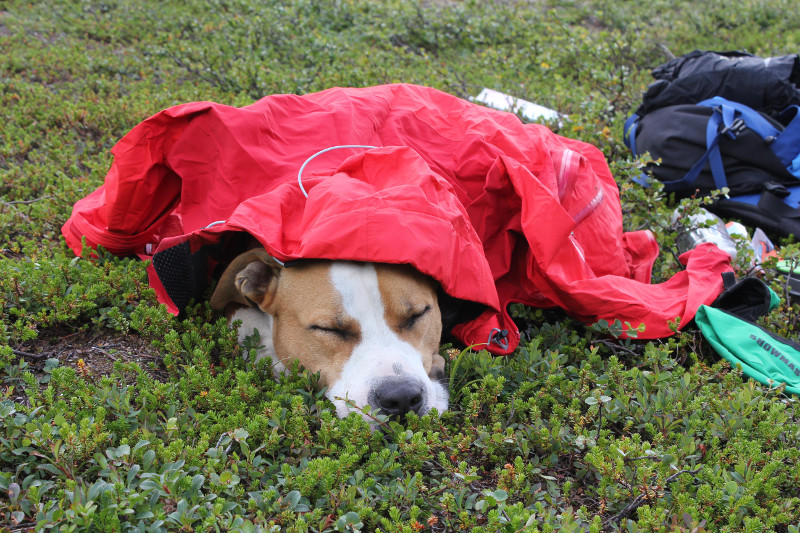
\includegraphics[width=0.6\textwidth]{hund_liten.jpg} \\
    \\
    \\
    {Författare} \\
    {\tt forfattare@student.ltu.se} \\
    {Institutionen för teknikvetenskap och matematik} \\
    \\ 
    
\includegraphics[width=0.2\textwidth]{ltu_swe.jpg}
    }

\date{\today} % Skriver ut dagens datum

\begin{document}

\maketitle % Genererar titel
\thispagestyle{empty} % Deklarerar sidans stil
%%%%%%%%%%%%%%%%%%%%%%%%%%%%%%%%%%%%%%%%%%%%%%%%%%%%%%%%%%%%%%
% -                  PREAMBLE SLUTAR HÄR                   - %
%%%%%%%%%%%%%%%%%%%%%%%%%%%%%%%%%%%%%%%%%%%%%%%%%%%%%%%%%%%%%%

%%%%%%%%%%%%%%%%%%%%%%%%%%%%%%%%%%%%%%%%%%%%%%%%%%%%%%%%%%%%%%
% -               Sammanfattning/Abstract                  - %
%%%%%%%%%%%%%%%%%%%%%%%%%%%%%%%%%%%%%%%%%%%%%%%%%%%%%%%%%%%%%%
\newpage % Varje huvudrubrik: \section{} ska börja på ny sida.
\pagenumbering{roman}

% Sammanfattning heter Abstract på engelska
\section*{Sammanfattning} % "*" tar bort numrering av titeln
Sammanfattningen är fristående från rapporten i övrigt. Man skall kunna läsa sammanfattningen utan att ha läst rapporten, och tvärtom. I sammanfattningen skall det finnas en kort beskrivning av problem, metod och de viktigaste resultaten samt vad de medför. Den skall vara komplett, objektiv och lätt att förstå. Sammanfattningen skall sammanfatta arbetet och någon extra information, som inte finns i rapporten, får inte skrivas in i sammanfattningen. Sammanfattningen skall vara kort och bör maximalt innehålla \numrange{150}{200}{} ord. Det ska inte finnas bilder eller figurer i sammanfattningen. Den bör inte innehålla referenser eller formler, men den ska beskriva de viktigaste resultaten.

%%%%%%%%%%%%%%%%%%%%%%%%%%%%%%%%%%%%%%%%%%%%%%%%%%%%%%%%%%%%%%
% -        Innehållsförteckning/Table of contents          - %
%%%%%%%%%%%%%%%%%%%%%%%%%%%%%%%%%%%%%%%%%%%%%%%%%%%%%%%%%%%%%%
\newpage % Ny sida
\tableofcontents % Skapar automatiskt en innehållsförteckning

%%%%%%%%%%%%%%%%%%%%%%%%%%%%%%%%%%%%%%%%%%%%%%%%%%%%%%%%%%%%%%
% -          Beteckningar/Nomenklatur/Nomenclature         - %
%%%%%%%%%%%%%%%%%%%%%%%%%%%%%%%%%%%%%%%%%%%%%%%%%%%%%%%%%%%%%%
\newpage
\section*{Beteckningar}
% Rapporter innehåller i allmänhet ett stort antal symboler och
% beteckningar som läsaren kan ha svårt att hålla reda på.
% Huvudregeln är att en storhet definieras och förklaras första
% gången den dyker upp i texten. Härutöver skall samtliga i 
% rapportens förekommande storheter, betecknade med latinska
% och/eller grekiska versaler och gemener, listas i en
% teckenförklaring.
\begin{table}[h] 
    \begin{tabular}{l l} % Två vänsterjusterade
    $\rho$ & Densitet (\si{kg/m^3}) \\
    $A$ & Area (\si{m^2})
    \end{tabular}
\end{table}

\newpage
\pagenumbering{arabic} 
\setcounter{page}{1}
%%%%%%%%%%%%%%%%%%%%%%%%%%%%%%%%%%%%%%%%%%%%%%%%%%%%%%%%%%%%%%
% -                 Inledning/Introduction                 - %
%%%%%%%%%%%%%%%%%%%%%%%%%%%%%%%%%%%%%%%%%%%%%%%%%%%%%%%%%%%%%%
\section{Inledning}
Inledningen introducerar läsaren till problemställningen och ger bakgrunden till problemet. Inledningen är viktig för det är här som läsaren skall ledas in i hur författaren tänkt. Hela avsnittet bör skrivas så att läsaren logiskt och motiverat leds fram till den problemställning som rapporten behandlar. I inledningen skall det finnas en översikt över närliggande tidigare arbeten inom ämnet, en så kallad litteraturstudie. Även här gäller att göra läsaren intresserad så att hen läser vidare i rapporten. Slutklämmen i inledningen bör göras så att det blir en mjuk övergång från Inledning till nästa kapitel.

Här är ett exempel med referenser: ``...kan beskrivas enligt \cite{Sterte2001}''.

Ange syftet med arbetet dvs vad som vill åstadkommas med arbetet, frågeställningar och vilka avgränsningar som finns. Målen skall vara specifikt klarlagda samt i rapportens slutsatser ska det tydligt framgå hur målen uppnåtts.

% Indelningen/Introduktionen kan med fördel indelas i
% underrubriker; 
% - Bakgrund, 
% - Problemformulering,
% - Litteraturstudie,
% - Syfte och mål, 
% - Avgränsningar.

% Lite skriv-vett
%
% 1. Använd aktiv form (vattnet strömmade genom röret). Det gör
% rapporten mer livlig.
% 2. Använd dåtid för observationer mm. Exempelvis ”ökat tryck
% gav större flöde”.
% 3. Använd nutid för generaliseringar och allmänt giltiga
% påståenden. Exempelvis ”I de flesta fall tillhör problemen kategorin
% olösbara problem”.
% 4. Undvik strunt, pompösa meningar och alla överdrifter.
% Uttryck som "utmärkt", "överensstämmelse" eller "fantastisk
% mätnoggrannhet" får inte förekomma.
% 5. Samtliga tidigare arbeten som åberopas i rapporten skall
% refereras till.
% 6. Skriv inte rapporten som en berättelse om vad ni gjort.
% 7. Berätta inte om de idéer som inte gav något.
% 8. Var mycket försiktig med negativa kommentarer om det egna
% arbetet.

%%%%%%%%%%%%%%%%%%%%%%%%%%%%%%%%%%%%%%%%%%%%%%%%%%%%%%%%%%%%%%
% -                       Teori/Theory                     - %
%%%%%%%%%%%%%%%%%%%%%%%%%%%%%%%%%%%%%%%%%%%%%%%%%%%%%%%%%%%%%%
\newpage
\section{Teori}\label{s:teori}
Beskriv teori, antaganden och annat som ligger till grund för den metod och det arbetssätt som valts. Teorin ska belysa/diskutera/sammanfatta och koppla till problemställningen. Samtliga ekvationer, figurer och tabeller ska numreras i löpande ordning. Figurer och tabeller ska ha en kortfattad text som klart och tydligt anger vad de visar, se Tabell~\ref{t:varme} och Figur~\ref{f:measurementdataonly}. Med figurer avses bilder, diagram, grafer mm. Det ska inte finnas ytterligare rubrik i figuren än den som står i figurtexten. Om ej egentillverkad skall källa anges samt tillstånd av ägare erhållas. Dessutom ska alla figurer och tabeller hänvisas till i den löpande texten. När man använder sig av \LaTeXe\ så anpassas tabellernas och figurernas position för att optimera textflödet då man kompilerar. Detta gäller även när man publicerar vetenskapliga artiklar. På engelska säger man att de är ``floats''.

När det gäller ekvationer så utgör de en del av texten, vilket innebär att kommatecken och punkter används precis som att ekvationen var ett antal sammansatta ord i texten. Variabler och parametrar skrivs med samma font både i ekvationerna och i brödtexten. Vanligtvis så uttrycks variabler och parametrar i $\mathbb{R}$ med hjälp av standardfont för matematik, t ex $x$ och $y$, medan vektorer och matriser oftast uttrycks med upprätt font i fet stil. Vi illustrerar detta med hjälp av nedanstående exempel, som också utgör den teoretiska grunden för tolkning av resultaten som presenteras i avsnitt~\ref{s:resultat}. Det finns många exempel på fysikaliska samband mellan en oberoende variabel $x$ och en beroende variabel $y=f(x)$ som approximativt kan beskrivas med hjälp av en potensfunktion på formen
%
\begin{equation} \label{e:potens}
    y=C x^k,
\end{equation}
%
där $C$ och $k$ kan bestämmas genom anpassning mot mätdata. Notera att i meningen ovan så läser man ekvationen som "...potensfunktion på formen $y$ är lika med $C$ gånger $x$ upphöjt till $k$, där $C$ och $k$ kan bestämmas...". Konstanterna $C$ och $k$ bestäms vanligtvis genom linearisera \eqref{e:potens} genom att logaritmera, dvs
%
\begin{equation}\label{e:logy}
    \ln y = \ln C + k \ln x.
\end{equation}
%
Om vi nu låter $\hat{z}=\ln y$, $w=\ln x$ och $m=\ln C$, så inser vi att \eqref{e:logy} att $\hat{z}(w)$ beskriver följande linjära samband
%
\begin{equation}\label{e:lin}
    \hat{z} = m + k w.
\end{equation}
%
Låt oss anta att vi har tre uppsättningar mätdata $(x_i, y_i)$, där $i=1\ldots3$ att tillgå. Genom att logaritmera mätdatat och att anta att det uppvisar en linjär relation så kan man använda teorin för potensfunktioner ovan tillsammans med minsta kvadratmetoden för att bestämma $k$ och $m$ i \eqref{e:lin}. Låt oss därför introducera matrisen $\mathbf{A}$ och vektorn $\mathbf{z}$ enligt
%
\begin{equation}
    \mathbf{A}=\begin{bmatrix}
    1&w_1\\
    1&w_2\\
    1&w_3
    \end{bmatrix},
~~~
    \mathbf{z}=\begin{bmatrix}
    z_1\\
    z_2\\
    z_3
    \end{bmatrix}.
\end{equation}
%
I vektornotation kan vi alltså uttrycka ${\hat{z}}$, som är en linjärkombination av kolumnerna i $\mathbf{A}$ som
%
\begin{equation}\label{e:zhat}
    \mathbf{\hat{z}}=\mathbf{A}\mathbf{a},
\end{equation}
%
där $\mathbf{a}=[m,k]^\mathrm{T}$. Minsta kvadratmetoden innebär att hitta den $\mathbf{a}$ som minimerar längden\footnote{Ländgen på en vektor i $\mathbb{R}^n$ bestäms av det euklidiska avståndet mellan dess start och ändpunkt.} på vektorn  mellan $\mathbf{\hat{z}}$ och vektorn $\mathbf{z}$. 

Vi inser att den vektor $\mathbf{e}=\mathbf{\hat{z}}-\mathbf{z}$ med det kortaste avståndet $e:=\|e\|=\|\mathbf{\hat{z}}-\mathbf{z}\|$ är den som är vinkelrät mot kolonnrummet\footnote{Planet som kolonnerna i $\mathbf{A}$ spänner upp.} till $\mathbf{A}$. Matematiskt innebär detta att
%
\begin{equation}\label{e:ATe}
    %\mathbf{A}\cdot\mathbf{e}=0 ~~~ \Longleftrightarrow ~~~ 
    \mathbf{A}^{T}\mathbf{e}=0.
\end{equation}
%
Eftersom att $\mathbf{e}=\mathbf{\hat{z}}-\mathbf{z}$ så har vi alltså
%
\begin{equation}\label{e:ATe1}
    \mathbf{A}^{T}\left(\mathbf{\hat{z}}-\mathbf{z}\right)=0
    ~~~ \Longleftrightarrow ~~~
    \mathbf{A}^{T}\mathbf{\hat{z}}=\mathbf{A}^{T}\mathbf{z}
    ~~~ \Longleftrightarrow ~~~
    \mathbf{A}^{T}\mathbf{A}\mathbf{a}=\mathbf{A}^{T}\mathbf{z}.
\end{equation}
%
Lösningen $\mathbf{a}$ till detta linjära system ges alltså av
%
\begin{equation}\label{e:a}
    \mathbf{a}=\left(\mathbf{A}^{T}\mathbf{A}\right)^{-1}\mathbf{A}^{T}\mathbf{z}.
\end{equation}
%
Slutligen kan vi bestämma $C=e^m$ genom att invertera $m=\ln C$ och vi alltså anpassat en potensfunktion av typen \eqref{e:potens} till mätdata.

\subsection{Teoriavsnitt ett}
Teoriavsnittet kan innehålla underrubriker. Kom bara ihåg att det alltid måste vara minst två, se avsnitt~\ref{s:teoriavsnitt2} nedan. 

När man presenterar variabler som representerar fysikaliska storheter så bör man även skriva ut deras enheter. Vanligtvis betecknar kraft $F$ och uttrycker dess enhet i Newton (N). Notera att ett mellanrum lämnas mellan det numeriska värdet och dess enheter. Undantag görs för procent (\%) och grader (\si{\degree}), som vanligtvis skrivs direkt efter det numeriska värdet, ex. $20$\% och $90$\si{\degree}.  Tyngkraften på grund av massan $m=$~\SI{100}{kg} ges av $F=mg$, där $g\approx$~\SI{9.82}{m/s^2} är tyngdaccelerationen. Tyngdkraften blir alltså $F\approx$~\SI{982}{N}.

\subsection{Teoriavsnitt två}\label{s:teoriavsnitt2}
Om man inte kan dela upp sitt avsnitt under minst två underrubriker, så använder man sig av paragrafer för att dela upp texten. Liksom figurer, tabeller och ekvationer så kan man referera till olika avsnitt i rapporten. I sektion avsnitt~\ref{s:metod} beskrivs härnäst hur man lämpligtvis presenterar den metoden man använt sig av.

%%%%%%%%%%%%%%%%%%%%%%%%%%%%%%%%%%%%%%%%%%%%%%%%%%%%%%%%%%%%%%
% -                       Metod/Method                     - %
%%%%%%%%%%%%%%%%%%%%%%%%%%%%%%%%%%%%%%%%%%%%%%%%%%%%%%%%%%%%%%
\newpage
\section{Metod}\label{s:metod}

Här beskrivs metoden, ofta är det lämpligt att dela upp texten i ett antal underrubriker. Använd alltid högst tre rubrik-nivåer.
Detta avsnitt delas ibland upp i metodbeskrivning, experimentell uppställning och/eller teoretiskt angreppsätt samt arbetsgång.

\subsection{Metodbeskrivning}
Att redogöra för sin metod är viktigt bland annat för att förklara varför den valda metoden ger ett tillförlitligt resultat. Alla antaganden och förenklingar måste anges och motiveras. Definiera matematiska modeller så att andra ingenjörer och forskare kan förstå vad du gjort.
Exempelvis utnyttjades MATLAB version 9.7 \cite{MATLAB2019} för att analysera mätresultatet som visas i Tabell~\ref{t:varme} samt plotta det linjäriserade datat och sambandet \eqref{e:lin} i Figur~\ref{f:analys}.

\subsection{Experimentell uppställning}

Alla eventuella försöksuppställningar beskrivs på ett sådant sätt att andra kan upprepa samma försök och verifiera dina resultat. Utnyttja figurer som förenklar din beskrivning.

\subsection{Experimentell procedur}
Kom ihåg att det alltid ska vara minst två underrubriker i varje avsnitt. Det gäller även om man delar upp avsnittet under en underrubrik i underrubriker.

\subsubsection{Mätmetod ett}
I denna studie användes två olika mätmetoder. Den första beskrivs i detta avsnitt.

\subsubsection{Mätmetod två}
Mätmetod nummer två...

%%%%%%%%%%%%%%%%%%%%%%%%%%%%%%%%%%%%%%%%%%%%%%%%%%%%%%%%%%%%%%
% -                    Resultat/Results                    - %
%%%%%%%%%%%%%%%%%%%%%%%%%%%%%%%%%%%%%%%%%%%%%%%%%%%%%%%%%%%%%%
\newpage
\section{Resultat}\label{s:resultat}

% Innehåll: resultat och analys.
% I vissa fall kan man ha ”Resultat och diskussion” som
% kapitel.

Detta är förmodligen den största delen av rapporten. Här redovisas resultaten rakt på sak på ett objektivt/neutralt sätt. Ofta är det lämpligt att dela upp texten i ett antal underrubriker. Materialet måste presenteras i logisk ordning, vilket inte behöver vara den ordning i vilken försöket/arbetet har utförts.

Läsaren skall kunna läsa rapporten utan att behöva bläddra fram och tillbaka. Det ska vara tydligt vad som är data respektive analys av data. Visas resultat i tabell- eller figurform så måste man i den löpande texten kortfattat beskriva vad man ser i figurerna/tabellerna. De placeras med fördel i närheten (efter) där de först refererades till, men med tanke på hur de hanteras vid typsättning så kan man inte garantera att de hamnar just där man helst vill att de ska vara. En konsekvens av detta är att man inte bör referera till dem som ``se Figur~\ref{f:analys} nedan'' eller ``Tabell~\ref{t:varme} ovan''. Man refererar rätt och slätt till dem med deras nummer och läsaren får lov att leta reda på var de befinner sig. Läsaren uppmanas nu att leta reda på Figur~\ref{f:analys} och Tabell~\ref{t:varme}. 

I Tabell~\ref{t:varme} innehåller uppmätta värden för kvarvarande värmemängd $\theta$ (J) vid fyra olika tidpunkter $t$ (s).
%
% Det skall alltid finnas en tabelltext som förklarar vad som
% finns i tabellen. Tabellnummer och text ska stå ovanför
% tabellen.
\begin{table}[ht]
\caption{Mätvärden för kvarvarande värmemängd $\theta$ vid ett antal olika tidpunkter $t$.}\label{t:varme}
\centering
    \begin{tabular}{c|cccccc}
        %\hline
        $t$ (s)       &6     & 35 & 47  & 87  & 145 & 329\\
        \hline
        $\theta$ (kJ) &3.10 &0.82 &0.60 &0.51 &0.28 &0.17
     \end{tabular} 
\end{table}
%
Figur~\ref{f:measurementdataonly} åskådliggör de uppmätta värdena för kvarvarande värmemängd vid tidpunkterna tabellerade i Tabell~\ref{t:varme} på två olika sätt. Till vänster i figuren återges nämligen rådatat och till höger så återges logaritmerat data.
%
\begin{figure}[!ht] % h=here t=top vilket är var vi helst skulle vilja 
% att den placerades. Kommandot \FloatBarrier kan också
% användas i koden för att begränsa hur långt bak en figur
% eller tabell hamnar i dokumentet.
%
\begin{center}
  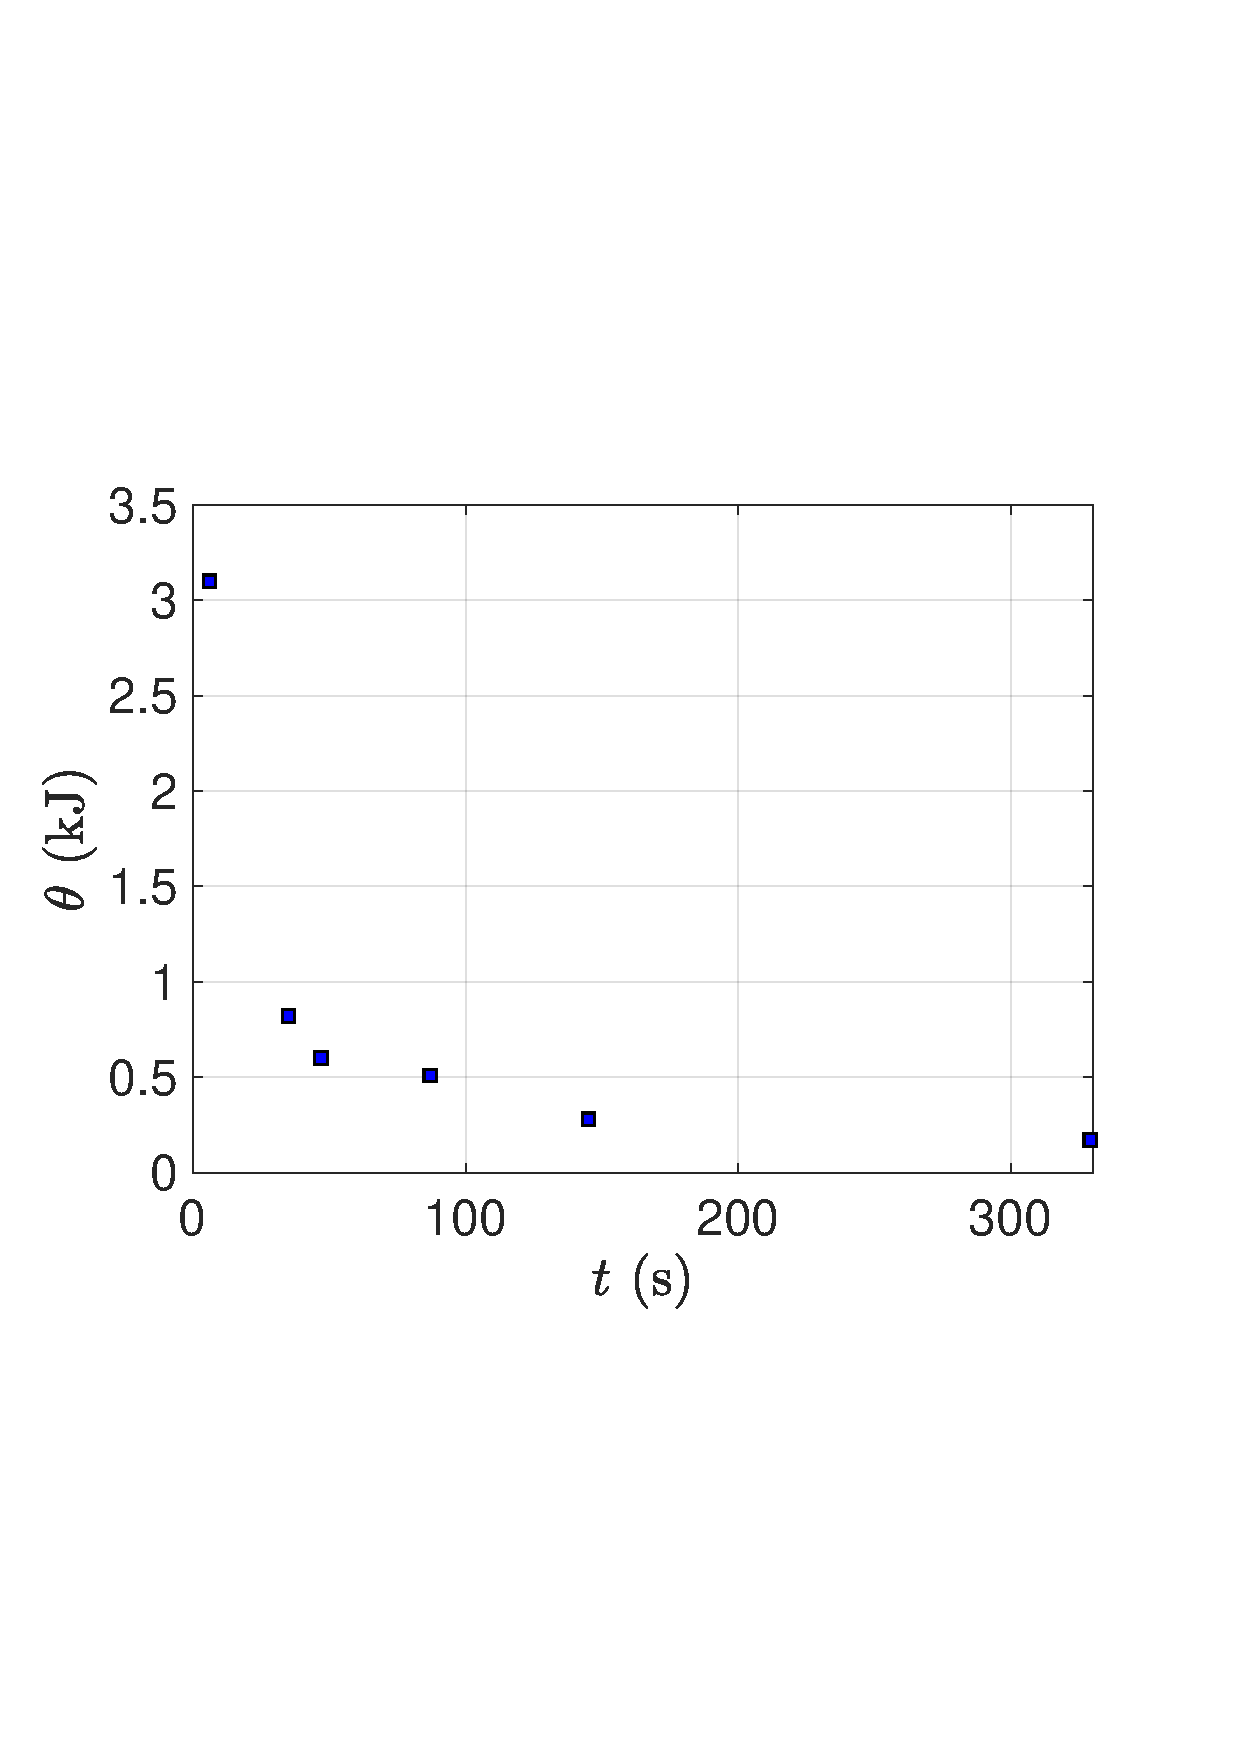
\includegraphics[width=0.5\textwidth,
  %trim={<left> <lower> <right> <upper>} 
   trim={0.7cm 7.5cm 1.2cm 6cm},clip]{measurementdataonly.pdf}~
   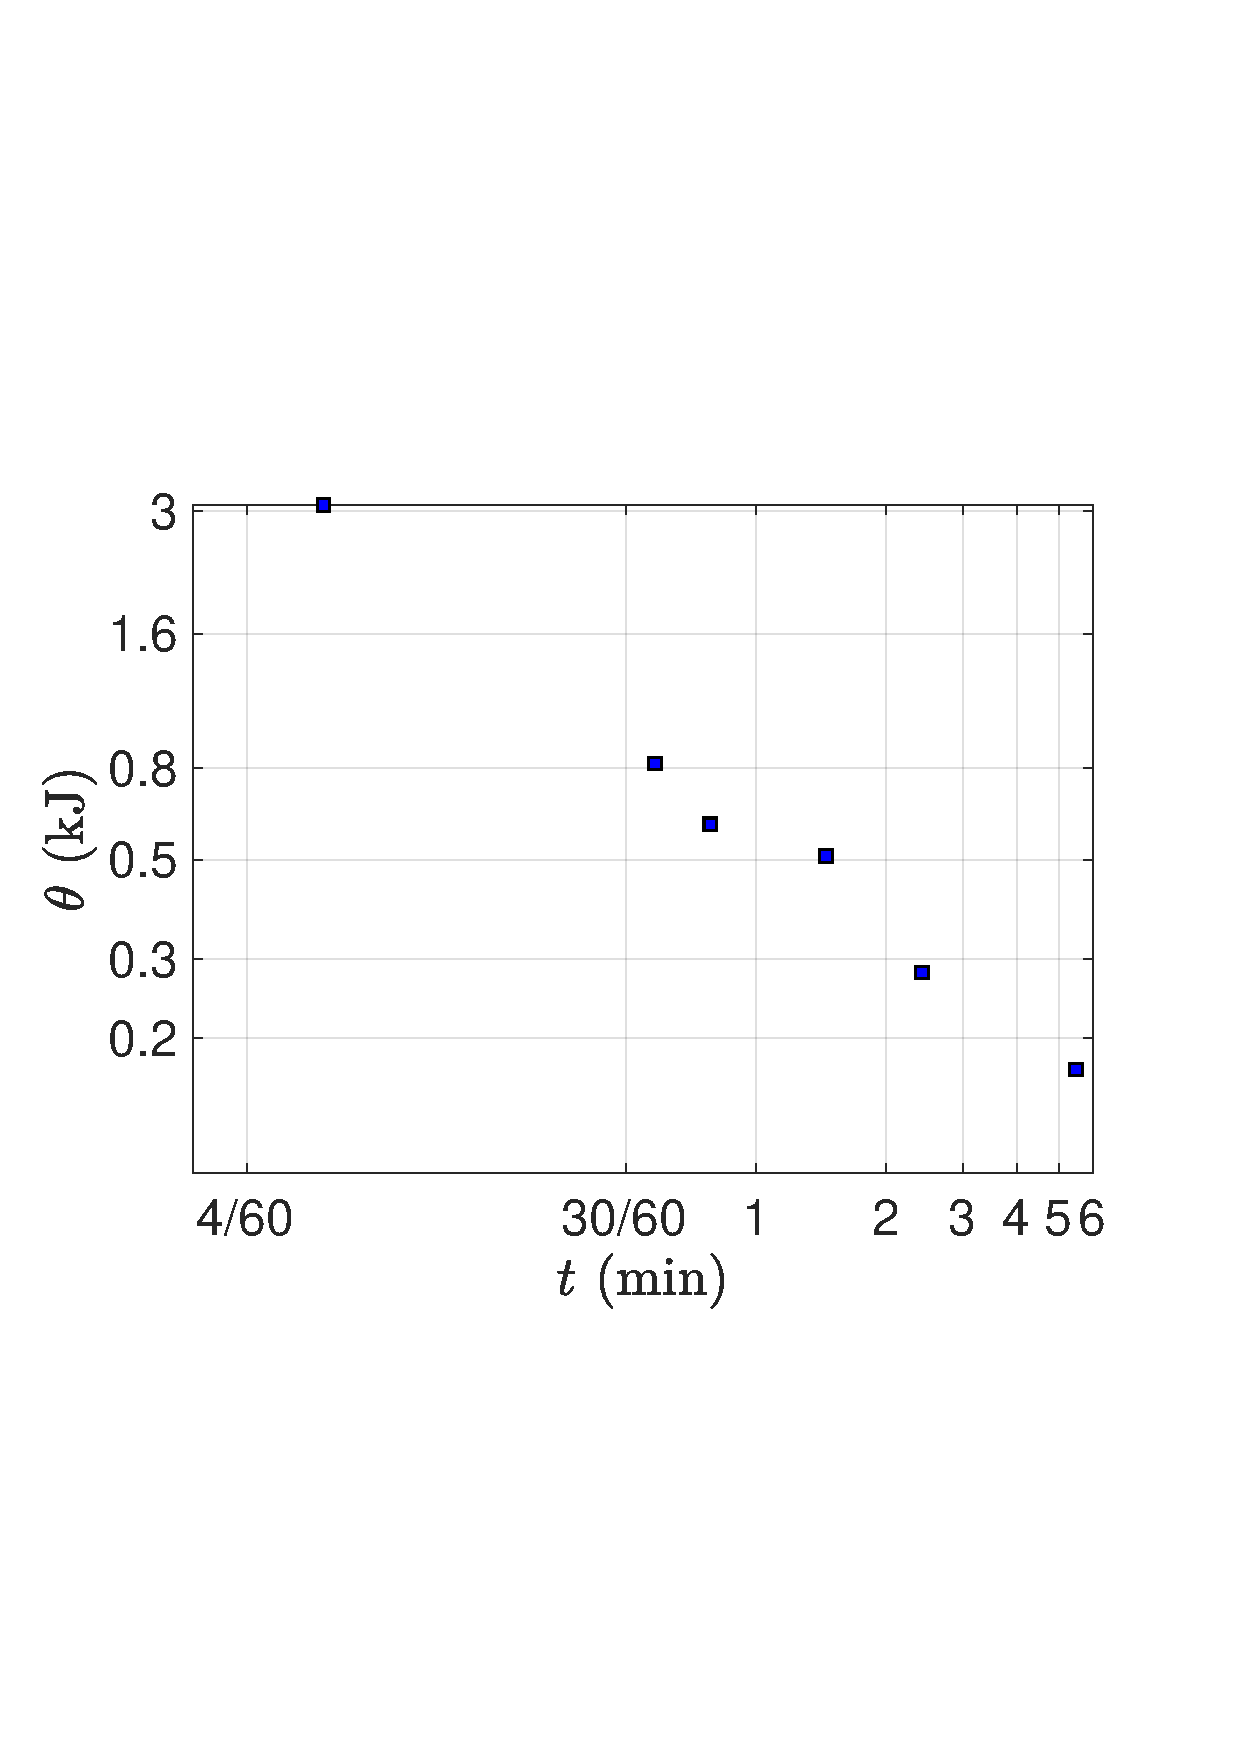
\includegraphics[width=0.5\textwidth,
  %trim={<left> <lower> <right> <upper>} 
   trim={0.7cm 7.5cm 1.2cm 6cm},clip]{logdata.pdf}
  \caption{Till vänster: uppmätta värden för kvarvarande värmemängd i vid ett antal tidpunkter. Till höger: logaritmerat data. \label{f:measurementdataonly}}
\end{center}
\end{figure}
%
Med hjälp av teorin i avsnitt~\ref{s:teori} och mätvärdena i Tabell~\ref{t:varme} anpassas en potensfunktion av typen
%
\begin{equation}
\theta = C t^k.
\end{equation}
%
Genom att använda minsta kvadratmetoden och då speciellt \eqref{e:a} kan vi bestämma $[m,k]^T$ till $[9.30,-0.72]^T$ med två decimalers noggrannhet. Det innebär således att 
%
\begin{equation}\label{s:linvarme}
    \hat{\theta}\approx 1100t^{-0.72}.
\end{equation}
%
Figur~\ref{f:analys} återger värdena för kvarvarande värmemängd i Tabell~\ref{t:varme} tillsammans med den anpassade potensfunktionen $1100t^{-0.72}$.
%
\begin{figure}[t] % h=here t=top vilket är var vi helst skulle
% vilja att den placerades
\begin{center}
  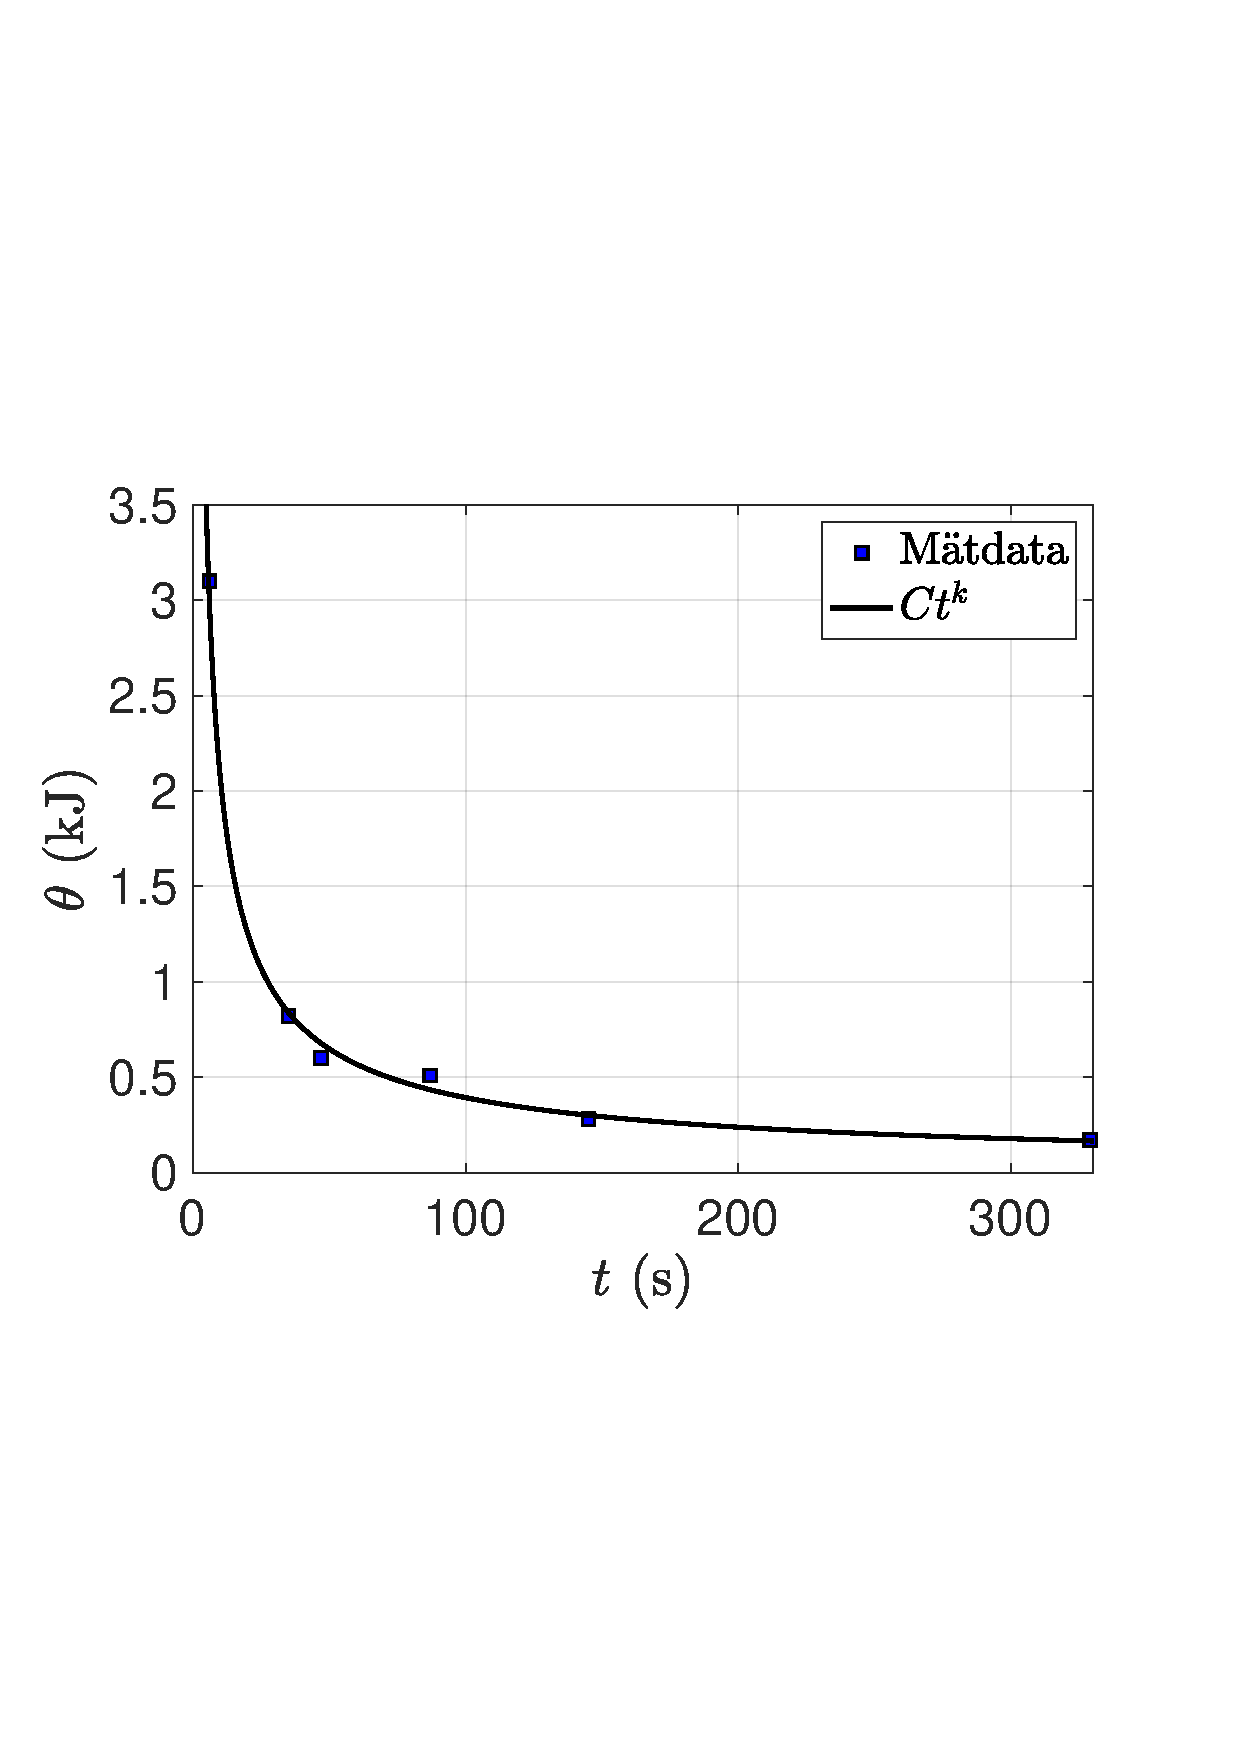
\includegraphics[width=0.6\textwidth,
  %trim={<left> <lower> <right> <upper>} 
   trim={0.7 7.5cm 1.2 6cm},clip]{analysis.pdf}
  \caption{Uppmätta värden för kvarvarande värmemängd i vid ett antal tidpunkter tillsammans med den anpassade potensfunktionen $1100t^{-0.72}$. \label{f:analys}}
\end{center}
\end{figure}
%
En vidare analys ger det relativa felet
%
\begin{equation}
    \frac{\|\hat{\mathbf{z}}-\mathbf{z}\|}{\|\mathbf{z}\|}\approx0.014
\end{equation}
%
% Diagram ska ha storhet och enhet på axlarna (SI). Är det tex
% logaritmerade diagram ska de ha storhet (men inte enhet) på
% axlarna.
% Figurnummer och text ska stå under figur och hänga ihop på
% samma sida.

För dem som är intresserade finns ett paket i \LaTeXe\ för att skapa grafer direkt i källfilen. Kolla på
\href{https://www.overleaf.com/latex/examples/latex-figures-using-tikzpicture-pgfplots-and-overpic/dffvyqktbcwk}{https://www.overleaf.com/latex/examples/latex-figures-using-tikzpicture-pgfplots-and-overpic}.

\subsection{Underrubrik ett vid behov}\label{s:resultatavsnitt1}
Har man en så måste man ha två.

\subsubsection{Underavsnitt även här om så behövs}
Men, har man en så måste man...

\subsubsection{Underavsnitt två till underavsnitt under huvudavsnitt}
...ha minst en till.

\subsection{Underrubrik två}
Denna ligger på samma nivå som underrubrik~\ref{s:resultatavsnitt1} och innebär att det finns minst två underrubriker till resultatavsnittet i denna rapport.

%%%%%%%%%%%%%%%%%%%%%%%%%%%%%%%%%%%%%%%%%%%%%%%%%%%%%%%%%%%%%%
% -             Diskussion och slutsater/Summary           - %
%%%%%%%%%%%%%%%%%%%%%%%%%%%%%%%%%%%%%%%%%%%%%%%%%%%%%%%%%%%%%%
\newpage
\section{Diskussion och slutsatser}

% Kan delas i separata kapitel: ”Diskussion” respektive
% ”Slutsatser”.
% Slutsatser skall vara korta och koncisa.
% Ibland är det lämpligast med indelningen ”Diskussion” samt
% ”Slutsatser och fortsatt arbete”

Här diskuteras (vad betyder/medför) resultaten utifrån ett vidare perspektiv och ställs i relation exempelvis till tidigare arbeten, referera i sådant fall till dessa. Utgående härifrån dras nödvändiga slutsatser som ska svara på de mål som angivits och vad resultaten har för relevans. Koppla slutsatser till uppställda mål. Diskutera felkällor och osäkerheter. Till exempel så skulle man här kunna nämna att ``det relativa felet på ca $1.4$\% antyder att potensfunktion $1100t^{-0.72}$ representerar den kvarvarande värmen med relativt god noggrannhet''.

Det är även lämpligt att i denna del avsluta med förslag och rekommendationer på fortsatta studier och undersökningar i ämnet. ``För att bättre kunna säkerställa approximationens noggrannhet behövs fler punkter mätdata''. Man kan dela upp diskussion, slutsatser och framtida studier i fristående kapitel.

%%%%%%%%%%%%%%%%%%%%%%%%%%%%%%%%%%%%%%%%%%%%%%%%%%%%%%%%%%%%%%
% -                  Referenser/Bibliography               - %
%%%%%%%%%%%%%%%%%%%%%%%%%%%%%%%%%%%%%%%%%%%%%%%%%%%%%%%%%%%%%%
\newpage
\printbibliography % Automatisk utskrift av referenslistan

% I denna del anges de källor du använt i ditt arbete. Ange 
% bara de viktigaste och alla referenser i listan måste vara
% refererade till i texten. I referenslistan får det inte
% förekomma någon referens som är ``allmänt bra att ha'' utan
% endast de referenser som författaren själv använt. Alla
% referenser ska refereras till i texten.
% OBS! använd originalreferenser. Undvik referenser till
% webbsidor eftersom de kan försvinna/ändras och kom ihåg att
% alltid skriva datum då sidan var tillgänglig i referensen.
%
% Ett av de vanligaste är att man skriver författarnamnet och
% sedan referensens publikationsår - det s.k. Harvard
% systemet.
% Exempel: ... även funnet av Charpak (1983)
% Är det två eller flera författare brukar man skriva
% Två författare: ... även funnet av Charpak och Öqvist
% (1983).
% Flera författare: ... även funnet av Charpak et al. (1983).
% ( et al. är latin (et alii) och betyder "och andra").
% 
% Ett annat sätt att ange en referens är att numrera
% referenserna i den ordning de dyker upp i texten och sortera
% referenslistan i nummerordning.
% Exempel: ... som Öqvist [3] har funnit, och referensen
% Öqvist dyker då upp som nummer tre i referenslistan.
% En guide för referenser finns här:
% http://libguides.ltu.se/skrivaoreferera

\end{document}
